\documentclass[tikz,border=8pt]{standalone}
\usepackage{amsmath,amssymb}
\usepackage{tikz}
\usetikzlibrary{arrows.meta}

\begin{document}
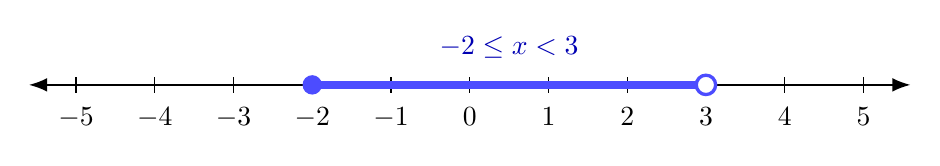
\begin{tikzpicture}[x=1cm]
  \draw[{Latex}-{Latex}, thick] (-5.6,0) -- (5.6,0);
  \foreach \x in {-5,...,5} {
    \draw (\x,0.1) -- (\x,-0.1) node[below=2pt] {$\x$};
  }
  \draw[line width=3pt, blue!70] (-2,0) -- (3,0);
  \fill[blue!70] (-2,0) circle (3.5pt);
  \filldraw[fill=white, draw=blue!70, line width=1.2pt] (3,0) circle (3.5pt);
  \node[above=6pt, blue!70!black] at (0.5,0) {$-2 \le x < 3$};
\end{tikzpicture}
\end{document}
